\pdfoutput=1


% RECOMMENDED %%%%%%%%%%%%%%%%%%%%%%%%%%%%%%%%%%%%%%%%%%%%%%%%%%%
\documentclass[graybox,natbib]{svmult}

% choose options for [] as required from the list
% in the Reference Guide
%% The amssymb package provides various useful mathematical symbols
\usepackage{amssymb,amsmath}

\usepackage{mathptmx}       % selects Times Roman as basic font
\usepackage{helvet}         % selects Helvetica as sans-serif font
\usepackage{courier}        % selects Courier as typewriter font
\usepackage{type1cm}        % activate if the above 3 fonts are
                            % not available on your system
%
\usepackage{makeidx}         % allows index generation
\usepackage{graphicx}        % standard LaTeX graphics tool
                             % when including figure files
\usepackage{multicol}        % used for the two-column index
\usepackage[bottom]{footmisc}% places footnotes at page bottom

\usepackage{url}
\usepackage[section,ruled]{algorithm}
\usepackage{algorithmic}
\usepackage{boxedminipage}
\usepackage[bookmarks=true,linkcolor=blue,hyperfootnotes=false,breaklinks=true,citecolor=blue,colorlinks=true]{hyperref}
\usepackage{sistyle}
\SIthousandsep{,}

% see the list of further useful packages
% in the Reference Guide

\makeindex             % used for the subject index
                       % please use the style svind.ist with
                       % your makeindex program

%%%%%%%%%%%%%%%%%%%%%%%%%%%%%%%%%%%%%%%%%%%%%%%%%%%%%%%%%%%%%%%%%%%%%%%%%%%%%%%%%%%%%%%%%

\begin{document}
\motto{Preprint submitted for \textbf{Learning Strategies and Cultural Evolution during the Paleolithic}, edited by Kenichi Aoki and Alex Mesoudi.  Please inform the authors about any citations prior to its print appearance.}
\title*{Behavioral Modernity and the Cultural Transmission of Structured Information: The Semantic Axelrod Model}
\titlerunning{Cultural Transmission of Structured Information}
% Use \titlerunning{Short Title} for an abbreviated version of
% your contribution title if the original one is too long
\author{Mark E. Madsen and Carl P. Lipo}
% Use \authorrunning{Short Title} for an abbreviated version of
% your contribution title if the original one is too long
\institute{Mark E. Madsen \at Dept. of Anthropology, University of Washington, Box 353100, Seattle, WA 98195 \email{mark@madsenlab.org}
\and Carl P. Lipo \at Department of Anthropology and IIRMES, California State University at Long Beach, 1250 Bellflower Blvd, Long Beach, CA  90840 \email{Carl.Lipo@csulb.edu}}
%
% Use the package "url.sty" to avoid
% problems with special characters
% used in your e-mail or web address
%
\maketitle



\abstract*{Cultural transmission models are coming to the fore in explaining increases in the Paleolithic toolkit richness and diversity. Social learning models may drive diversity through  relaxation of conformism, population growth, or the effects of extinction and recolonization in metapopulations. During the Paleolithic, however, technologies increase not only in terms of diversity but also in their complexity and interdependence. As \citet{Mesoudi2008a} have shown selection broadly favors social learning that is hierarchical and structured, rather than information which is piecemeal and independent. The addition of structured information acquisition potentially explains how the complexity of technology changes along with diversity. Here, we introduce a structured extension of the Axelrod model of cultural differentiation (1997). We examine the conditions under which structured suites of traits develop and differentiate in the model, which can represent the chains of prerequisites, “background” information, and local specializations characteristic of real technology traditions. Our results point to ways in which we can build more comprehensive explanations of the archaeological record of the Paleolithic as well as other cases of technological change.}

\abstract{Cultural transmission models are coming to the fore in explaining increases in the Paleolithic toolkit richness and diversity. Social learning models may drive diversity through relaxation of conformism, population growth, or the effects of extinction and recolonization in metapopulations. During the Paleolithic, however, technologies increase not only in terms of diversity but also in their complexity and interdependence. As \citet{Mesoudi2008a} have shown selection broadly favors social learning that is hierarchical and structured, rather than information which is piecemeal and independent. The addition of structured information acquisition potentially explains how the complexity of technology changes along with diversity. Here, we introduce a structured extension of the Axelrod model of cultural differentiation (1997). We examine the conditions under which structured suites of traits develop and differentiate in the model, which can represent the chains of prerequisites, “background” information, and local specializations characteristic of real technology traditions. Our results point to ways in which we can build more comprehensive explanations of the archaeological record of the Paleolithic as well as other cases of technological change.}


\section{Introduction}\label{introduction}

Although humans and our hominid ancestors have been cultural animals
throughout our evolutionary history, an important change occurred in our
lineage during the Middle and Upper Paleolithic. After many millennia
with varied but relatively small toolkits, and material culture which
was very similar across continental distances, our cultural repertoire
began to explode. The artifactual toolkit became larger and its
constituent tools and technologies more complex, the range of materials
used to construct it was enriched, and our solutions to the problems of
everyday life became regionalized and differentiated. Further, the
economic basis of our lives began to broaden and also, in many areas, to
become specialized \citep{bar2002upper, d2011evolution, guy2005mosaic}
This transition has long been called the ``Upper Paleolithic
Revolution,'' or less humbly, even the ``Human Revolution'' by those who
see such characteristics as marking out what it means to be uniquely
human.

Careful examination of the Middle Paleolithic archaeological record,
especially in Africa and the Near East, suggests that this change in
behavior was not a sharp ``revolution,'' and that much of the enriched
material culture we later characterize as the ``Upper Paleolithic'' had
precursors in many areas. These were patchy, both in space and time
\citep{bouzouggar200782, d2007additional, d2011evolution, guy2005mosaic, mcbrearty2000revolution, mcbrearty2007down}.
Nevertheless, even if our understanding of the time scale over which
this enrichment occurred has lengthened and the spatial scope has
widened, it remains a central puzzle in the evolution of our species. As
a neutral term, we prefer ``behavioral modernity,'' which emphasizes a
pattern or phenomenon, not its timing, geography, or association with
biology.

The most promising explanations of behavioral modernity are those which
examine the nature of cultural variation and social learning itself, and
factors which might lead to the evolution of more diverse populations.
Several possibilities have already been explored. Shennan
\citetext{\citeyear{shennan2000population}; \citeyear{shennan2001demography}}
proposed that demography has a powerful effect on diversity within
cultural transmission processes, and this seems to be supported by the
reduced cultural diversity and loss of toolkit elements observed in
Tasmania during a population bottleneck \citep{henrich2004}. But a
recent comparative study shows that population size itself bears no
relationship with toolkit diversity \citep{collard2013risk}. If simple
transmission models do show a relation between diversity and population
size, it is likely to be a second-order effect in the real world,
dominated by or interacting with other factors.

The structure of bands or demes into larger regional metapopulations,
however, is a first-order effect, given what we know about the strong
effect that network topology has upon contagion or diffusion processes
\citep[e.g.,][]{castellano2009statistical, smilkov2012influence}. Premo
\citeyearpar{premo2012local} has examined whether metapopulation
dynamics, with local extinction and recolonization, might account for
the retention and expansion of diversity, with promising results.
Finally, the way social learning occurs within a population can
radically change its quantitative results over time. Sharon
\citeyearpar{sharon2009acheulian} suggested that Middle Paleolithic
populations might have been characterized by strongly conformist
learning, which changed over time, leading to a dramatic increase in
cultural diversity.

A foundational event in human evolution like behavioral modernity is
highly unlikely to have a single cause, especially if it evolved over
many tens of millennia in a widely distributed population. Instead, we
should expect a combination of factors. Demography, and the
metapopulation dynamics of individual demes or groups likely played
roles, with the strength of such effects depending upon localized
circumstances. The way in which individuals learn skills and information
likely plays a central role. And we cannot forget the strategic
dimension of social life: the evolution of cooperation and pro-social
behaviors are probably implicated as well. Sterelny
\citeyearpar[p.61]{sterelny2012evolved} sums up the multi-factor view
nicely:

\begin{quote}
\ldots{}the cultural learning characteristic of the Upper Paleolithic
transition and later periods of human culture---social transmission with
both a large bandwidth and sufficient accuracy for incremental
improvement---requires individual cognitive adaptations for cultural
learning, highly structured learning environments, and population
structures that both buffer existing resources effectively and support
enough specialization to generate a supply of innovation.
\end{quote}

We believe this is a promising approach. A useful next step is to
construct formal models which incorporate some of these factors, and
determine if their dynamics exhibit the kind of qualitative changes we
see in the transition from archaic to behaviorally modern assemblages.
Specifically, we need models which:

\begin{itemize}
\itemsep1pt\parskip0pt\parsep0pt
\item
  Represent cultural traits as hierarchically structured, in order to
  study increases in complexity
\item
  Have learning rules sensitive to the structure and relations of
  cultural traits
\item
  Have mechanisms (such as homophily) which allow cultural
  differentiation endogeneous to the model
\end{itemize}

As the ``learning environment'' in such models is tuned from lower to
higher fidelity, we would expect to see greater diversity, larger
structured sets of traits persisting in the population, and greater
differentiation of the population into ``different'' cultural
configurations.

In this chapter, we introduce a simulation model which combines a
hierarchical trait space capable of expressing the ``semantics'' of
relationships between skills and information \citep{Mesoudi2008a}, and a
modified version of Robert Axelrod's \citep{axelrod1997} homophilic
social learning model which allows us to examine these expectations.
Models like this begin to move beyond diffusion dynamics, bringing the
actual meaning and relations of traits into the modeling process. Hence
we call these ``semantic Axelrod'' models, and believe that such models
form a platform for formalizing the type of multi-factor hypotheses
necessary to examine major transitions in human evolution, such as
``behavioral modernity.'' After describing the model, we study its
dynamics and provide an initial assessment of its suitability for
studying the onset of behavioral modernity in the later Paleolithic.

\section{The Semantic Axelrod Model for Trait
Prerequisites}\label{the-semantic-axelrod-model-for-trait-prerequisites}

Much of our technical knowledge, whether of stone tool manufacture,
throwing clay pots, or computer repair, is built from simple tasks, bits
of background knowledge, and step-by-step procedures
\citep{neff1992ceramics, schiffer1987theory}. We organize our knowledge
and skills in many ways, but it common to think of a complex process as
a ``script'' or ``recipe'' \citep{schank1977scripts}. Of course, experts
in a task or field may not see it this way, having internalized such
structures below the conscious level. Experts will often know more than
one way to accomplish any given goal, and be able to repurpose and
recombine methods and tools, as opposed to the simpler, more linear or
tree-based recipes of the novice or student.
\citep[e.g.,][]{Bleed:2008in, bleed2002obviously, stout2002skill}.

A detailed formal model of the relations between steps in a
technological process, or the knowledge necessary to execute a
technological recipe, will involve many kinds of relations. Some items
will be related in time, as steps in a process. Others will be related
by subsumption: arrowheads are a subclass of bifacial stone tools, and
require many of the same production techniques as bifaces used in other
projectiles. Still others will be related as sets of alternatives:
choices of surface treatment for a given ceramic paste, given the firing
regime selected, for example. Models of stone tool production often use
sequences to represent the relations in a construction recipe, but
models such as trees or more general graphs are possible and
usefulArchaeologists have frequently organized the relations between
these skills and production steps into ``sequence models'' or
``$\textrm{cha\^ine op\'eratoire}$,'' but many representations are
possible, including trees
\citep{Bamforth:2008kq, Bleed:2008in, Ferguson:2008ce, Hogberg:2008fj, bleed2001trees, bleed2002obviously, schiffer1987theory, stout2002skill}.

In this chapter, we focus not on the execution steps of a recipe, but
the relations between skills and information \emph{as it is learned}. In
other words, we focus upon the \emph{prerequisite} relationships that
exist between cultural traits, since these govern the way in which
social learning is constrained in the environment of learning and
teaching. Some pieces of information or skills must be in place before a
person can effectively learn or practice other. Examples from our own
childhoods abound: one needed to understand addition and subtraction and
multiplication before learning long division; in order to make soup, we
need to understand how to simmer rather than boil, how to chop and
slice, what ingredients might be combined, and so on. The fact that
knowledge and skills build upon one another make prerequisite relations
between cultural traits ubiquitous. Incorporating such relations into
social learning models is thus a useful first step in understanding how
the human cultural repertoire changed in the later Paleolithic. We
represent prerequisite relations as trees in the graph-theoretic sense
\citep{diestel2010graph}, replacing the ``flat'' structure of
``local/allele'' models or the ``dimension/mode'' structure of
classifications and some typologies \citep{Dunnell1971}.

Our model also requires a way of representing a changing learning
environment, in ways that create higher fidelity and greater possibility
for building cumulative knowledge. In real learning envrionments, there
are many possibilities, but deliberate teaching, and apprentice learning
are repeatedly seen across human groups as ways that naive individuals
can reliably learn the complex skills and information needed for
foraging, artifact production and maintenance, and navigating an
increasingly rich social world. The point of structuring the learning
environment with teaching and/or apprenticeship is to give the learner
skilled models to imitate, shortcut trial and error when acquiring a
skill, provide a reference for needed information, and to guide
individuals to put their information and skills together into
appropriate sequences to accomplish an overall goal. Apprenticeship and
formalized teaching provide a social learning ``scaffold'', helping to
lower the amount of individual trial and error learning needed to master
a body of material \citep{wimsatt2007reproducing, wimsatt2007re}.

Within a standard discrete-time simulation model of a social learning
process, we can model this type of learning environment with the
following modifications:

\begin{enumerate}
\def\labelenumi{\arabic{enumi}.}
\itemsep1pt\parskip0pt\parsep0pt
\item
  Disallowing individuals the ability to copy traits for which they
  don't have necessary background or prerequisites.
\item
  Creating a probability that individuals, if disallowed a trait, may be
  able to learn one of its necessary prerequisites instead, leading to
  the possibility of full acquisition at some future time.
\end{enumerate}

By changing the probability that individuals learn a missing
prerequisite trait, we can ``tune'' the learning environment. Low
probabilities might correspond, for example, to a learning environment
where individuals can observe others executing a production step, but
are given little or no instruction or guidance on what they need to know
in order to successfully master it. High probabilities of learning
prerequisites would correspond, on the other hand, to environments where
individuals receive instruction, or work together with a more skilled
individual who guides them toward learning the information and skills
they lack. In the next section, we discuss the implementation of both
points in more detail.

\subsection{Representation of Traits And Their
Prerequisites}\label{representation-of-traits-and-their-prerequisites}

In order to represent the ``prerequisite'' relations between a number of
cultural traits, we organize the traits into trees\footnote{A tree is a
  graph with no cycles or loops. That is, a tree is a connected graph on
  $n$ vertices that possesses at most $n-1$ edges
  \citep{diestel2010graph}. Furthermore, in this chapter we are
  concerned with \emph{rooted} trees, in which one vertex is
  distinguished as the ``origin'' of the tree, giving rise to a
  hierarchical structure.}, where nodes higher in the tree represent
knowledge, skills, or concepts which are necessary for traits further
down the tree. Let us consider the different skills and information
necessary for the construction of a single artifact, say a dart thrown
by an atlatl. An artisan will possess information about different raw
materials, an understanding of what materials are suitable for specific
purposes, skills and information concerning the knapping of different
types of bifaces, methods of hafting bifaces into different kinds of
shafts, and so on. Here, we are interested in the order in which people
usually \emph{learn}, rather than the order in which steps are executed.
Thus, nodes closer to the top of a tree are ``background'' or necessary
skills to nodes further down in a tree. For example, a basic
understanding of the properties of stone would occur close to the root
of a tree, while knowledge of the differences between specific sources
of lithic raw material would occupy nodes at the same level below the
root.

In each simulation model, we begin with a trait or ``design space'' that
incorporates several independent sets of prerequisite relations
\citep{o2010cultural}. This models the fact that some knowledge is
always independent and can be learned in parallel, since it may relate
to different aspects of a process. For example, one might learn about
the sources of good lithic raw materials, independent of learning how to
perform different percussion techniques. The overall design space of a
simulation model is thus a forest\footnote{A forest is a graph composed
  of multiple components, each of which is a tree.}, composed of several
trees.

\begin{figure}[htbp] 
\centering 
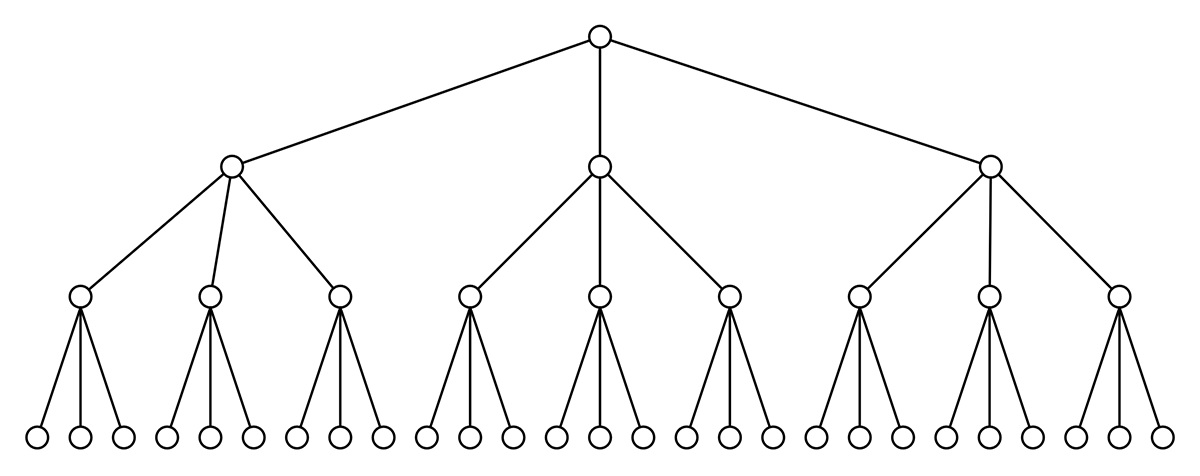
\includegraphics[]{balanced-trait-tree-3-3.png} 
\caption{A single trait tree, represented by a balanced tree with branching factor 3 and depth factor 3, order 40.  In our model, nodes higher in the tree represent prerequisites for nodes lower down the tree.  Each instance of the model will have several or many of these trees in the design space.} 
\label{img:trait-tree} 
\end{figure}

We employ balanced trees which have the same number of nodes at each
level, to provide a simplified model of a design space with which to
begin our exploration of this class of social learning model, although
real design spaces are undoubtedly more complex in their geometry. Each
tree in our model is specified by a branching factor $r$ and depth $h$.
As a result, each trait tree in the design space has
$\sum_{i=0}^{h} r^i$ traits. The tree depicted in Figure
\ref{img:trait-tree} thus has 40 vertices, for example. In this chapter,
we examine both small (4 trees) and larger (16 trees) design spaces, to
see how learning may differ in problems involving design spaces of
different size and complexity. We examine trees with combinations of
branching and depth factors of 3 and 5. Thus, a design space with 4
trees with branching and depth factors of 3 (as in Figure
\ref{img:trait-tree}) would have 160 traits, whereas a design space with
16 trees of branching and depth factors of 5 would have a total of
62,496 traits.\footnote{We initially chose 6 as the limit on branching
  and depth factors, but found that we cannot calculate certain
  symmetric statistics, such as the size of the automorphism group, on
  trees that large using existing tools. Even a tree with $r=5, h=6$ has
  over $10^{1623}$ possible symmetries, and calculating that number
  takes over 100 seconds on a fast multi-core computer.} Even the small
design spaces we consider here create a large space for cultural change
and differentiation, given the number of possible trees one can
construct on even 40 vertices.\footnote{If we consider each trait to be
  unique and non-interchangeable, the number of unique trees with unique
  vertex labels is $n^{n-2}$ by Cayley's theorem
  \citep{diestel2010graph}. For example, for each trait tree of 40
  vertices, there are roughly $10^{60}$ possible trees. Even if we
  consider traits to be interchangeable (e.g., we look at the abstract
  topology of trees rather than the details of individual traits), there
  are \emph{at least} $10^{16}$ possible unlabelled rooted trees on 40
  vertices (using Otter's \citeyearpar{otter1948number} approximation).}

Given the total ``design space'' represented by a forest of trait trees,
each individual in our model is initialized with a small number of
``initial'' traits. Initial traits are chosen randomly but heavily
weighted towards the roots of the trees to represent the fact that our
knowledge starts out basic and sparse. In the next sections we describe
the social learning model, modified from Robert Axelrod's original, by
which each simulated population evolves within this tree-structured
design space, and will return to the specifics of how an initial culture
repertoire is chosen.

\subsection{The Axelrod Model of Social Learning and
Differentiation}\label{the-axelrod-model-of-social-learning-and-differentiation}

Robert Axelrod \citeyearpar{axelrod1997} formulated a model aimed at
studying the conditions under which simple learning rules could lead to
cultural differentiation, rather than a single fixed state (which is the
result of simpler neutral or diffusion models). This makes it useful as
a starting point for understanding phenomena such as behavioral
modernity, in our view. Axelrod's model combines social learning, in the
form of random copying, a spatial structure to interaction, in the form
of localized copying of neighbors on a lattice, and the tendency to
interact most strongly with those to whom we are already culturally
similar (homophily). The model displays a rich and interesting set of
behaviors, and has been extensively studied by social scientists and
physicists \citep{castellano2009statistical}. First we review the basic
model, and in the following section our modified algorithm.

\subsubsection{Axelrod's Original Model}\label{axelrods-original-model}

The original model locates $N$ individuals on the nodes of a regular
lattice or grid, but various network structures have also been studied.
Each individual is endowed with $F$ integer variables
$(\sigma_1,\ldots,\sigma_F)$, that can each assume $q$ values. In the
original model, each variable is a ``cultural feature'' each of which
can assume $q$ ``traits.'' In each step, a randomly chosen individual
$i$ and a random neighbor $j$ are selected, and ``interact'' with
probability equal to the overlap between their cultural repertoire.
Overlap, in the basic model, is simply the fraction of features for
which $i$ and $j$ possess the same trait value:

\begin{equation}\label{eq:axelrod}p(i,j) = \frac{1}{F} \sum_{f=1}^{F} \delta_{\sigma_f(i)\sigma_f(j)}\end{equation}

where $\delta_{i,j}$ is Kronecker's delta function, taking the value $1$
when its two arguments are equal and $0$ otherwise. When individuals
interact, the focal individual $i$ takes the trait value of its neighbor
for one of the features where the two individuals differ.

Interaction has no effect when two individuals already possess identical
cultural repertoires, and there is no probability of interaction if
individuals have no traits in common. This eventually causes the model
to reach an absorbing state where no further changes are possible.
Instances of the model are initialized with a random distribution of
traits among individuals, and left to update until the steady state is
reached. The evolution of the population leads to two classes of
absorbing states: (a) a ``monocultural'' state in which all individuals
share the same set of variables, and (b) a ``polycultural'' state in
which subpopulations exist which share the same set of variables within
the group, and are completely different from their neighbors.

Which of the two results is reached, and the statistical character of
``polycultural'' states when they exist, depends mainly upon the number
of traits possible $q$ for each cultural feature. For small values of
$q$, individuals share many traits with their neighbors, interactions
are thus frequent, and one domain comprising a single set of traits will
grow to become fixed within the entire population. In contrast, when the
value of $q$ is high, individuals start out sharing very few traits,
with interactions that are correspondingly less frequent. Regions of
uniform cultural variation do grow, but as they do, sets of individuals
who share no traits at all (and thus do not interaction) grow as well,
and often prevent any single regional culture from expanding to fix
within the population.

Many variants of the basic Axelrod model have been studied, including
the addition of ``drift'' via the introduction of copying error,
situating agents on different types of complex networks, the addition of
an external ``field'' to simulate the effects of mass media, and copying
that obeys a ``conformist'' or majoritarian rule by selecting the most
common trait among the neighbor set
\citep{castellano2000nonequilibrium, de2009effects, flache2006sustains, GonzalezAvella:2007p6910, GonzalezAvella:2007p6912, gonzalez2005nonequilibrium, gonzalez2006local, Klemm:2003p7031, Klemm:2003p7112, Klemm:2005tb, Lanchier:2010p16999, Lanchier:2012ur}.
In general, modifications of the basic model can reduce the tendency of
the model to produce polycultural solutions, or change the time scale or
location of the critical point.

\subsubsection{Semantic Extensions to the Axelrod
Model}\label{semantic-extensions-to-the-axelrod-model}

We begin each simulation with $N$ (100, 225, or 400) agents, arranged on
a square grid. A design space is created, with some number of trait
trees (4 or 16), with uniform branching factors and depth factors (3 or
5). An example of such a tree is shown in panel A of Figure
\ref{img:prereq}. Initial traits (and their prerequisites) are chosen
randomly across the configured number of trait trees, as follows. For
each individual, we select a random number $t$ between 1 and 4, and
repeat the trait selection process $t$ times for that individual. In
each selection, we choose a random tree in the design space, and then
select a depth in the tree for the trait, given by
$d  \sim \textrm{Poisson}(0.5)$. This biases trait selection towards the
root of the tree, as one would expect in young or inexperienced
individuals. We then walk $d$ steps into the tree, making uniform random
selections for the children of each vertex. The path of vertices thus
constructed is added to the individual's trait set, giving them an
initial trait and its necessary prerequisites. One such initial trait is
shown in Panel B of Figure \ref{img:prereq}. Given that individuals
begin with a small number of initial traits (between 1 and 4, selected
randomly), and their prerequisites, the initial trait endowment of an
individual is between 1 and $4h$, where $h$ is the maximum depth of the
design space (either 3 or 5 in the experiments reported here).\footnote{The
  median number of traits in samples taken after 6-10 million time steps
  is considerably higher--259 traits per cultural configuration or
  region. Thus, cultural repertoires grow significantly over time, as
  expected.}

\begin{figure}[htbp] 
\centering 
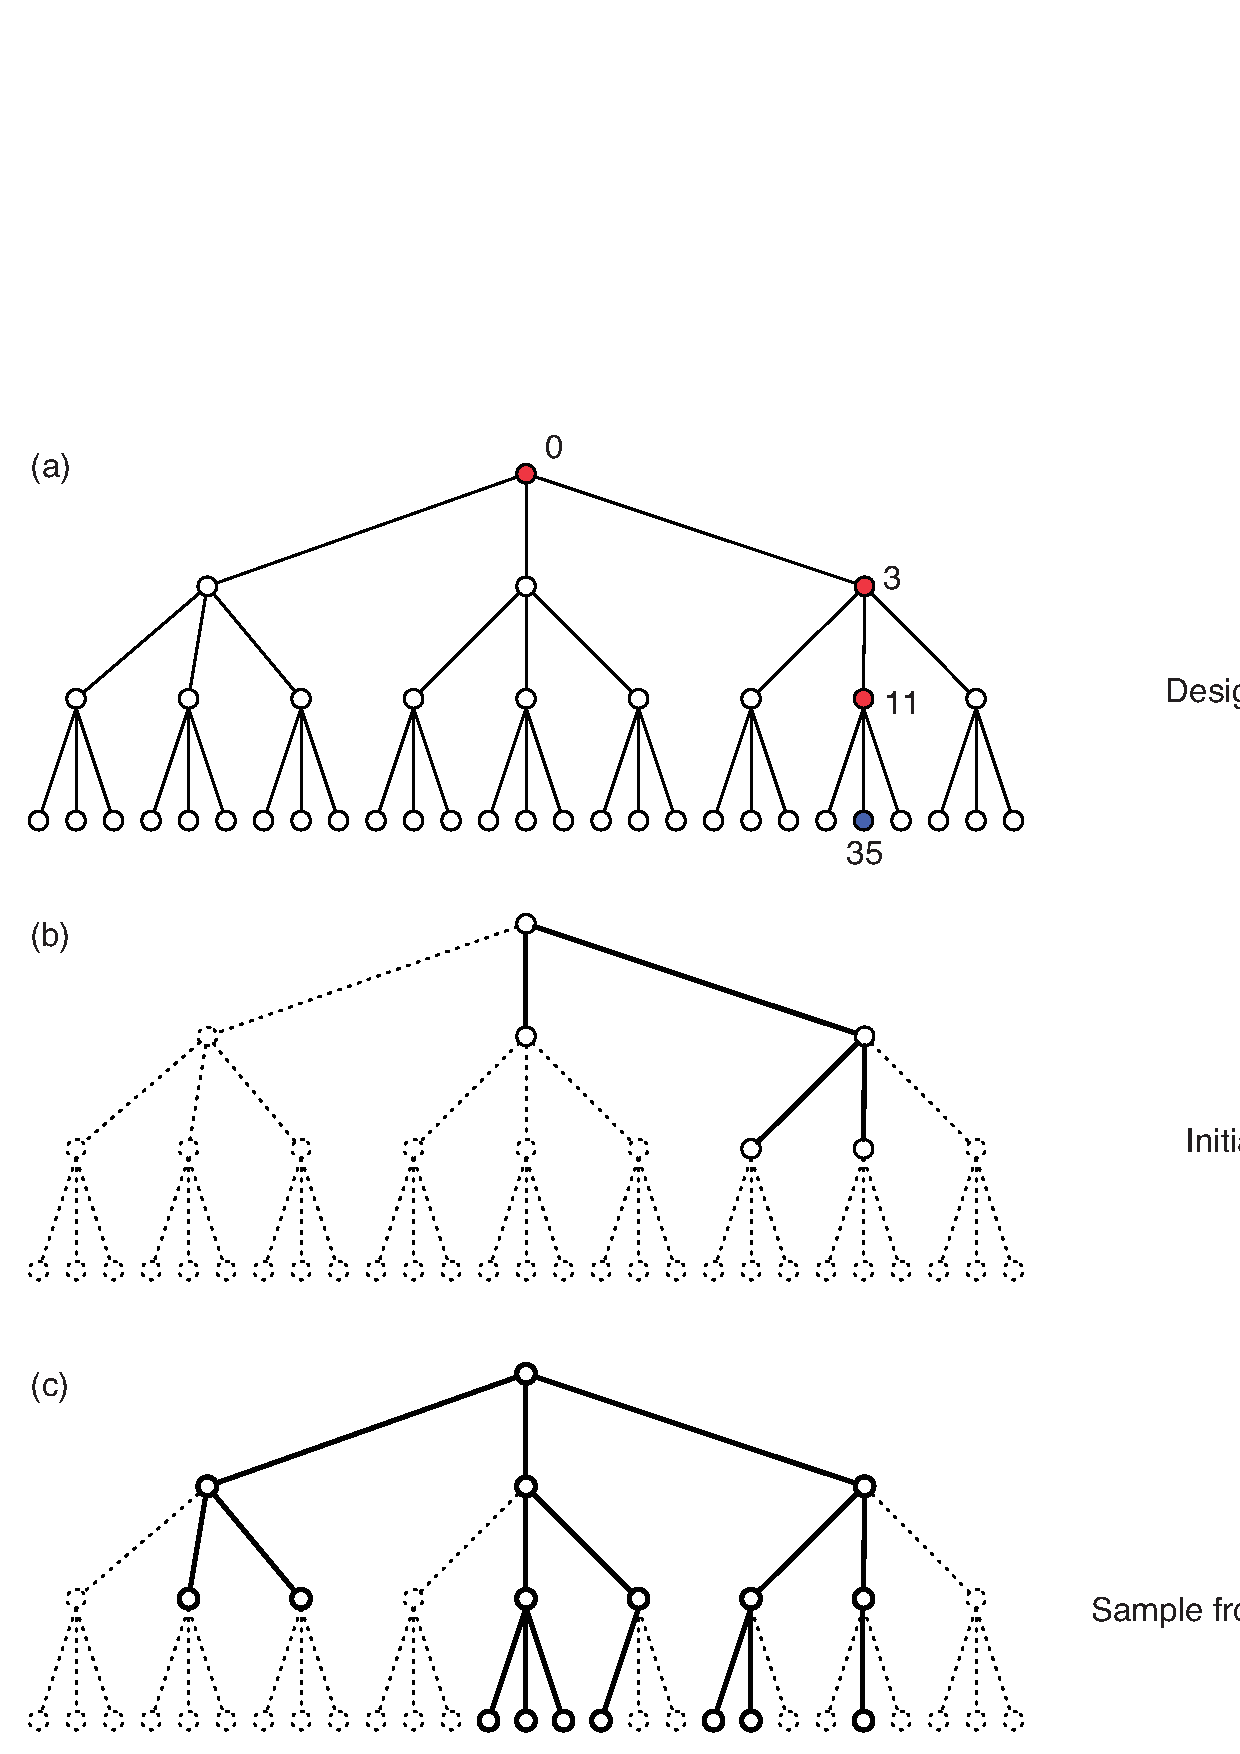
\includegraphics[scale=0.5]{design-init-final.pdf} 
\caption{Illustration of a design space composed of a single trait tree, along with a random initial trait chosen from the design space, and a final sample from a simulation run, showing the evolution of traits within the design space.  Also shown in the top panel are the ``prerequisites'' for a cultural trait (35), as an example.} 
\label{img:prereq} 
\end{figure}

Once the population is initialized, the simulation runs a discrete
approximation to a continuous-time model. In other words, only one agent
changes at each elemental time step, as in the original Axelrod model
and the Moran model of population genetics and its cultural version
\citep{aoki2011rates, moran1962statistical, moran1958random}. At each
step, an agent (A) is chosen at random, and a random neighbor of A is
then selected (agent B). Their probability of interaction is given by
the overlap of trait sets, which is most simply calculated as the
Jaccard overlap between the set of tree vertices each possesses, thus
replacing Equation \ref{eq:axelrod} with:

\begin{equation}J(A,B) = \frac{|A \cup B| - |A \cap B|}{|A \cup B|}\end{equation}

If the agents end up interacting, agent A randomly selects a trait from
B which it does not already possess. If agent A has the necessary
prerequisites for the desired trait (T), it learns the trait
immediately, adding T to its repertoire. If not, it cannot immediately
learn T, but there is a learning rate parameter for the simulation run
which governs the chance that agent A will instead learn one of T's
prerequisites during this time step. Given a learning event, we again
walk from the root of the tree down the path towards the trait T,
finding the first trait in the path that Agent A does not already
possess. For example, agent A might require the trait closest to T
(e.g., trait 11 in Figure \ref{img:prereq}, if the original trait
targeted was 35).

Additionally, at each time step, there is a probability that one
individual, chosen randomly, will learn a new trait (and necessary
prerequisites) that it does not already possess. This simulates the
ongoing process of individual learning unconnected to social learning
within the population, as well as the process of individual innovation.
Because this functions much like ``infinite-alleles mutation'' in the
classical Wright-Fisher neutral models \citep{Ewens2004}, or like noise
terms in Axelrod, Ising, or Potts models
\citep{castellano2009statistical}, we will refer to this as the
``mutation'' rate in this chapter.

Each simulation run lasts 10 million steps, which is an average of
100,000 copying events per individual (in a population of
100).\footnote{100,000 was chosen as a compromise for running large
  batches of simulations in parallel. Some simulation runs, especially
  in small design spaces with very high prerequisite learning rates, can
  converge to a monocultural solution and quasi-stable equilibrium quite
  quickly; in the largest design spaces and low learning rates,
  convergence may never occur even though the process is well-mixed.
  However, the processes have reached a quasi-stable equilibrium,
  verified by examining samples at different times for secular trends in
  median and mean values, which were not found.} Samples are taken
beginning at 6 million steps, and sampling at an interval of 1 million
steps, and record the trait trees seen in the population. An example of
such a sampled tree is shown in Panel C of Figure \ref{img:prereq}. For
reference, the full algorithm for each copying step is given in the
Appendix as Algorithm \ref{alg:tree-prereq-axelrod}.

\section{Measuring Cultural Diversity and the Results of Structured
Learning}\label{measuring-cultural-diversity-and-the-results-of-structured-learning}

Each sample from a simulation run is composed of the distinct sets of
trait trees possessed by individuals in the population, along with
summary statistics. If a simulation run converges to a monocultural
solution, the sample will have one set of trait trees, which are shared
across the entire population. In other cases, there will be multiple
cultural configurations or ``regions,'' which might be unique to a
single individual, or shared by some number of agents. Each region will
be composed of some number of trait trees (typically, the number
configured for the simulation run: 4 or 16, but perhaps a subset), and
each trait tree will be the result of many agents learning traits and
their prerequisites socially, and for runs with a non-zero mutation
rate, by individual learning or innovation. Each culture region will
thus have some number of traits, typically higher (often much higher)
than the initial endowment given to the population.

\begin{figure}[htbp] 
\centering 
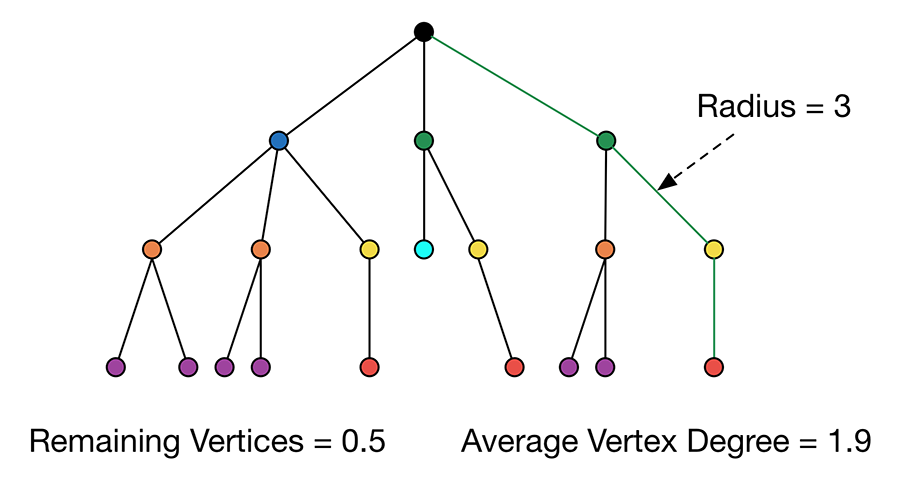
\includegraphics[]{equil-trait-tree.png} 
\caption{An example set of traits at the conclusion of a simulation run, extracted from a simulation with branching factor 3 and depth factor 3, and a single trait tree as the trait space.  The remaining density of vertices, mean vertex degree, and radius of the tree are noted.  Vertex colors denote ``structural equivalence'' classes or ``orbit structure,'' as measured by adjacency patterns, and is one measure of the symmetries present in the tree.} 
\label{img:final-tree} 
\end{figure}

Samples contain descriptive statistics for the trait trees of each
cultural region, as follows. The ratio of the number of traits in the
sample to the full design space size (or ``remaining density'' of
traits) is a measure of how diverse a cultural region is. The radius of
a rooted tree is the number of edges in the path from root to the
furthest edge. The average radius of trees in a sample (or its ratio to
the depth of the design space) is a measure of how diverse and ``deep''
a cultural configuration is. Similarly, in the original design space,
the branching factor describes how many children each node in the tree
started with, so measuring the average vertex degree gives us a rough
measure of how diverse the cultural configuration is (in terms of
breadth)\footnote{This is an approximate measure, compared to radius,
  because the leaves of a tree have no children, and thus the mean
  degree of the design space is slightly less than the branching factor
  of the tree (plus one, because every vertex does have a parent node).
  This can be made more precise by calculating the actual mean degree of
  the original design space, but we have not done so here.}. Each of
these measures is illustrated in Figure \ref{img:final-tree} for an
example tree selected from our data.

In addition to these simple numerical measures comparing final trees to
the original design space, it is useful to measure something about the
overall ``shape'' of the trees themselves. One way of formalizing this
notion is to examine the \emph{symmetries} of the final trait trees.
Examining Figure \ref{img:final-tree}, if we ignore the exact identities
of traits for the moment, it is apparent that there are repeating
patterns. For example, the left-most branches each terminate in a pair
of leaves. This pattern is repated on the second right-most branch.
These types of repeating patterns are computationally expensive to
search for in large sets of trees, but we can summarize them by
considering trait trees as algebraic objects and examining their
\emph{automorphisms}.

An automorphism is a function which maps an object to itself, in such a
way that the structure of the object is preserved
\citep{rotman1995introduction}. Graph automorphisms map vertices in a
graph to each other, preserving properties such as the adjacency pattern
of edges. The six vertices which mark the repeating pattern of
leaf-pairs in Figure \ref{img:final-tree} are an automorphism of the
tree, and thus are symmetries we can measure. An overall measure of
``how symmetrical'' (or ``how many interchangeable patterns'') there are
in a graph possesses given by the total number of automorphisms found,
called the size of the automorphism group or $|\textit{Aut}(G)|$
\citep{godsil2001algebraic}. A tree with no repeating patterns will thus
have an automorphism group size of 1, indicating that the only symmetry
is the entire tree itself. A balanced tree with branching and depth
factors of 3, as depicted in Figure \ref{img:trait-tree}, has
approximately $1.3 \times 10^{10}$ automorphisms. The more repeating
patterns there are in trait trees, the more automorphisms they will
possess.

Because group sizes grow quickly and the accuracy of performing
calculations with truly astronomical numbers is low, another possible
measure of the symmetries present is to count the \emph{classes} of
equivalences into which vertices fall. The \emph{orbits} of the
automorphism group are the sets of vertices which are interchangable by
some permutation that preserves structure. For example, the graph in
\ref{img:trait-tree} has five orbits, with each vertex at a given level
interchangable (in a structural sense). Similarly, the six leaf vertices
that are part of pairs in Figure \ref{img:final-tree} are part of the
same orbit; in this illustration, each orbit is given a different color
to highlight their equivalence. For each cultural region found when
sampling a simulation, we calculate the size of the automorphism group
and the number and multiplicity (frequency) of orbits. For this
analysis, we employ the \emph{nauty + Traces} software by Brendan McKay
and Adolfo Piperno \citep{McKay201494}.\footnote{Nauty+Traces can be
  downloaded at \url{http://pallini.di.uniroma1.it/}. We employed
  version 2.5r7 for this research.}

\section{Experiments}\label{experiments}

For this chapter, we examined populations of size 100, 225 and 400, to
begin to examine the effects of population size. For these populations,
we examined design spaces that were small (4 trait trees) and large (16
trait trees). Within each size, we further examined combinations of
branching factor and depth factor with values of 3 and 5, thus yielding
8 total sizes of design space (Table
\ref{tab:axelrod-design-space-size}).

\begin{table}[H]
\begin{tabular}{|c|c|c|c|}
\hline
\textbf{Branching Factor} & \textbf{Depth Factor} & \textbf{Number of Trait Trees} & \textbf{Size of Design Space}\\ 
\hline
3 & 3 & 4 & 160\\ 
\hline 
5 & 3 & 4 & 624\\ 
\hline 
3 & 5 & 4 & 1456\\ 
\hline 
5 & 5 & 4 & 15624\\ 
\hline 
3 & 3 & 16 & 640\\ 
\hline 
5 & 3 & 16 & 2496\\ 
\hline 
3 & 5 & 16 & 5824\\ 
\hline 
5 & 5 & 16 & 62496\\ 
\hline 
\hline
\end{tabular}
\caption{Size of design space for different trait tree configurations}
\label{tab:axelrod-design-space-size}
\end{table}

Further, we examined three levels of global mutation or innovation rate:
zero, or no mutation, and 0.00005 and 0.0001. Such rates created a
constant supply of new innovations, but several orders of magnitude less
frequent than copying and prerequisite learning events. The full set of
parameters are given in Table \ref{tab:axelrodct-sim-parameters}. For
each combination of all of the above parameters, we performed 25
replications.  With 5 samples per simulation run, this yielded 10,963,691 samples of cultural regions.  

\begin{table}[H]
\begin{tabular}{|p{0.6\textwidth}|p{0.4\textwidth}|}
\hline
\textbf{Simulation Parameter} & \textbf{Value or Values} \\ 
\hline
Population rate at which new traits arise by individual learning & 0.0, 5e-05, 0.0001\\ 
 \hline 
Maximum number of initial traits (not including their prerequisites) each individual is endowed with & 4\\ 
 \hline 
Number of distinct trees of traits and prerequisites & 4, 16\\ 
 \hline 
Population sizes & 100, 225, 400\\ 
 \hline 
Replicate simulation runs at each parameter combination & 25\\ 
 \hline 
Maximum time after which a simulation is sampled and terminated & 10000000\\ 
 \hline 
Individual probability for learning a missing prerequisite & 0.05, 0.1, 0.2, 0.3, 0.4, 0.5, 0.6, 0.7, 0.8, 0.9\\ 
 \hline 
Number of branches at each level of a trait tree & 3, 5\\ 
 \hline 
Depth of traits in each trait tree & 3, 5\\ 
 \hline 
\hline
\end{tabular}
\caption{Parameter space for simulations described in this chapter}
\label{tab:axelrodct-sim-parameters}
\end{table}



The simulations were designed to examine whether the combination of a
hierarchical, tree-like representation of cultural traits, in
combination with an Axelrod-like model which provides the possibility of
cultural differentiation, is a good platform for exploring questions
surrounding behavioral modernity. We are not experts concerning
Paleolithic assemblages, so our efforts are exploratory, and an attempt
to construct models which can be extended and applied to real data.

In analyzing the results of the semantic Axelrod model described here,
we looked at the degree to which individuals converged in their cultural
repertoire (as we might describe conditions in the early Paleolithic),
or under what conditions did social learning lead to greater individual
variation in repertoires? This is measured by the number of cultural
regions in samples of the population taken at quasi-stationary
equilibrium.

Second, we looked at whether highly structured learning environments,
represented here by higher probabilities of naive individuals gaining
the prerequisites for the skills and information they encounter with
peers, led to deeper and richer cultural repertoires. We also began
examining whether there are invariant statistical properties of those
repertoires, through the use of symmetry measures. The measures used are
those described above: the tree radius (or depth), mean vertex degree,
the fraction of remaining vertices, and the size of the automorphism
group of sampled trait forests. Finally, we began to examine how the
structured learning environment might interact with demography, by
simulating the same parameters across two sizes of population.

\section{Results}\label{results}

We begin by noting that compared to the original Axelrod model, or
neutral and biased copying models, the dynamics of our semantic axelrod
model are highly variable. A very wide range of outcomes is possible for
each parameter combination, especially when the size of the design space
is large. Some variables, such as the average vertex degree of sampled
trait trees, strongly overlap across all learning rates and are not
considered further in this chapter. Given the large amount of
variability in the dynamics, larger numbers of replications would be
useful, although this is computationally quite expensive at
present.\footnote{The simulations reported here ran on a cluster of 6
  compute-optimized ``extra large'' Linux instances on Amazon's EC2
  computing cloud, for a total of 17 days of wall clock time and 2075
  CPU hours. We plan further optimizations to the simulation code to
  make larger samples economically feasible.} That said, several
features of the data are strongly suggestive that hierarchical trait
models have potential in modeling cumulative technological evolution,
making the computational expense worthwhile.

\subsection{Cultural Diversity}\label{cultural-diversity}

Variation among individuals is foundational to evolutionary processes,
and is the raw material from which differentiation between regions and
cultural groups is constructed. In the simulations reported here, we
examine diversity within a single population, but we are planning a set
of metapopulation experiments with the same model to address regional
diversification. In Figure \ref{img:size-spectrum-cultures-100} we show
the size spectrum of cultural regions (clusters of individuals with the
same trait trees), for each combination of prerequisite learning rate
and design space size. The variable plotted here is the number of
cultural regions in a given sample. Thus, in a population of size 100,
if there is 1 cultural solution, then all 100 individuals share it. If
there are 100 cultural regions, then every individual had a unique
configuration of cultural traits. In the lower left corner are the very
lowest learning rates, in small design spaces. We believe this could
correspond to the kind of learning environments and knowledge structures
that characterizes human technology through much of the early and middle
Paleolithic. In this corner, most cultural regions span the entire
population (given the large spike on the left). In small design spaces,
configurations become more diverse and smaller on average, as the
learning rate increases. As it becomes highly probable that an
individual will learn the prerequisites they need for an encountered
skill or trait, the population fragments among different portions of the
design space.

\begin{figure}[htbp] 
    \centering
    \includegraphics[scale=0.4]{size-spectrum-regions-saa12full.pdf}
    \caption{The sizes of cultural configurations, by the size of the design space (horizontal), and prerequisite learning rate (vertical), for population size 100.}
    \label{img:size-spectrum-cultures-100}
\end{figure}

Two other effects are also visible in these data. First, the
distributions become bimodal for most combinations of design space size
and learning rate. The left hand peak corresponds to simulation runs
which had no global innovation or mutation rate, and where only copying
and prerequisite learning occurred. In such populations, cultural
regions were uniformly large and populations quickly converged on a
single set of traits. This highlights the importance of various
``innovation'' and ``invention'' processes in the creation and
maintenance of cultural differentiation and diversity
\citep{eerkens2005cultural, o2010innovation}, and suggests that
systematic change in innovation processes may be a crucial component of
any multi-factor model for the evolution of behaviorial modernity. The
second effect is the distinctive narrowing of the size distribution in
the largest design spaces and highest learning rates. This is not an
artifact of the length of time into the simulation run a sample was
taken, since the distributions look identical for samples taken at 1
million step intervals. This is likely just the signature of a small
population evolving in a very large design space. This effect warrants
further study, since it may be a source for group divergence as
information and technology accumulates in human societies.

\subsection{Trait Richness and Knowledge
Depth}\label{trait-richness-and-knowledge-depth}

\begin{figure}[h] 
\centering 
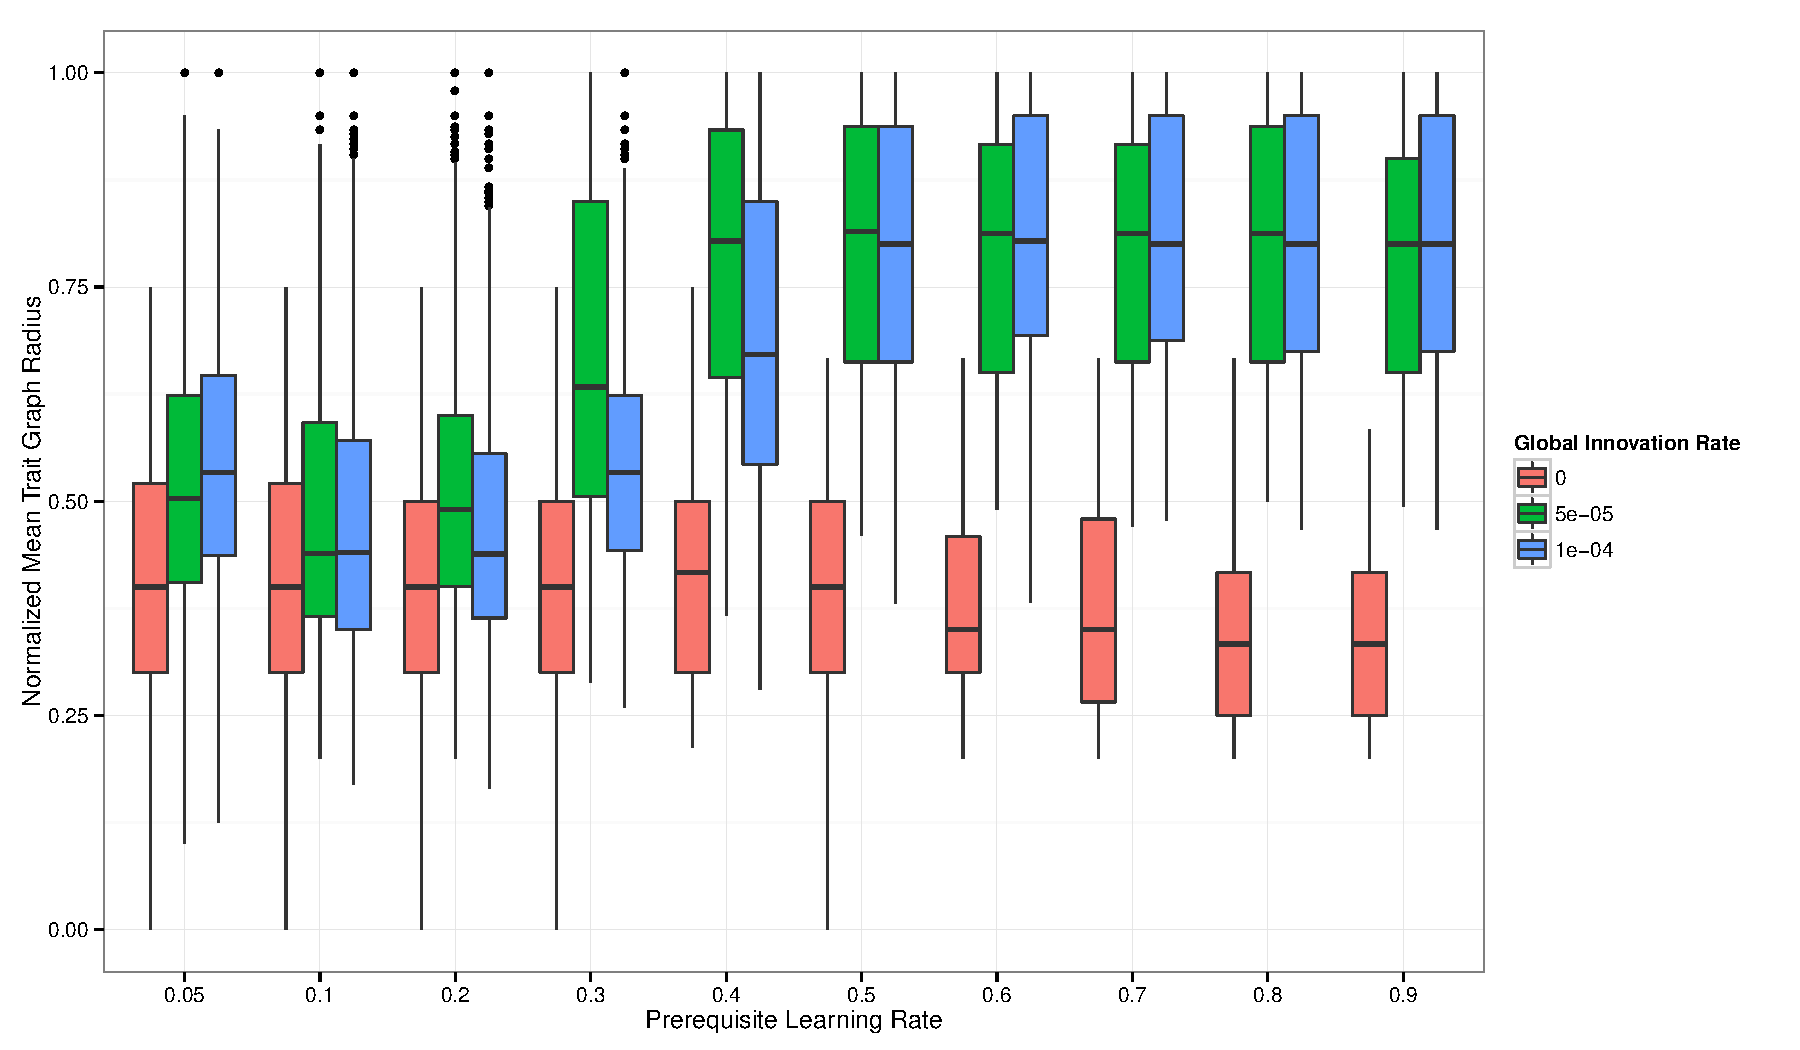
\includegraphics[scale=0.4]{mean-radius-by-learning-rate-innov-12.pdf} 
\caption{Mean depth of trait sets, by prerequisite learning rate and global innovation rate, for population size 100.} 
\label{img:mean-radius-cultures-100} 
\end{figure}

Cumulative evolution of technology is represented in our model by the
population learning its way \emph{down} the trees which compose the
design space. Possession of traits deeper in the trees represents skills
or information which is more specific, possessing more prerequisites.
Thus, we expect that the depth (or ``radius'', see Figure
\ref{img:final-tree}) of trees would increase with the prerequisite
learning rate, representing a learning environment which is structured
to ensure such acquisition.

Figure \ref{img:mean-radius-cultures-100} gives the \emph{normalized}
mean radius of cultural regions, broken out by the prerequisite learning
rate along the horizontal axis, and each group of 3 boxplots displays
the differing global innovation rates studied. Radii are normalized to
the depth of their design space, to facilitate comparison. The results
indicate that essentially two regimes exist: shorter trees, which do not
grow much beyond their initialized size, and larger trees. The mean
radius has an asymptote just above 0.75, achieved with the prerequisite
learning rate is approximately 0.4 or higher. Further increases do not
seem to matter. Additionally, the difference between the two global
innovation rates is small--what matters most in terms of qualitative
behavior is the presence of global innovation outside the teaching or
learning of prerequisites themselves.

\subsection{Population Size}\label{population-size}

Earlier, we mentioned that population size does not seem to be a primary
factor in explaining the measured diversity in cultural transmission
models, except perhaps in bottleneck situations like the one Henrich
analyzes in Tasmania \citeyearpar{henrich2004}. Instead, population size
may have an interaction effect with other factors, yielding smaller
second-order effects. We examined the effect of population size in the
research reported here, repeating the entire set of simulation runs for
populations of 100, 225, and 400.\footnote{We should note that learning
  rates of 0.8 and 0.9 for population size 400 were cut short due to
  budget constraints, but this does not appear to affect the pattern in
  our dataset.}

\begin{figure}[h] 
\centering 

\includegraphics[scale=0.4]{mean-radius-by-learning-rate-pop.pdf} 
\caption{Mean depth of trait sets, by prerequisite learning rate and population sizes of 100, 225 and 400.} 
\label{img:mean-radius-cultures-pop} 
\end{figure}

Figure \ref{img:mean-radius-cultures-pop} displays the relationship
between mean radius (or depth) of the cultural traits in each cultural
sample, as in Figure \ref{img:mean-radius-cultures-100} above, but the
boxplots are instead colored by population size. There is no qualitative
difference in the dynamics as sample size grows, but the mean radius of
trait sets does decline slightly, probably due to the slower velocity at
which an innovation diffuses in the larger population. This is the kind
of second-order effect which warrants continuing to include population
size in analyses of social learning models, we believe, even if it does
not serve as a primary explanation or factor.

\subsection{Trait Tree Symmetries}\label{trait-tree-symmetries}

Finally, we examined the algebraic properties of the trait trees
composing cultural regions, examining both the number of vertex
equivalence classes (orbits) and the size of the automorphism group of
the trait forests. We examined the raw metrics, and versions normalized
by the size of the maximally symmetric forest with the same number of
traits, branching factor, and depth factor. The latter proved difficult
and led to serious overflow problems even with 64 bit arithmetic, so we
focus here on the raw automorphism group size.

\begin{figure}[h] 
\centering 
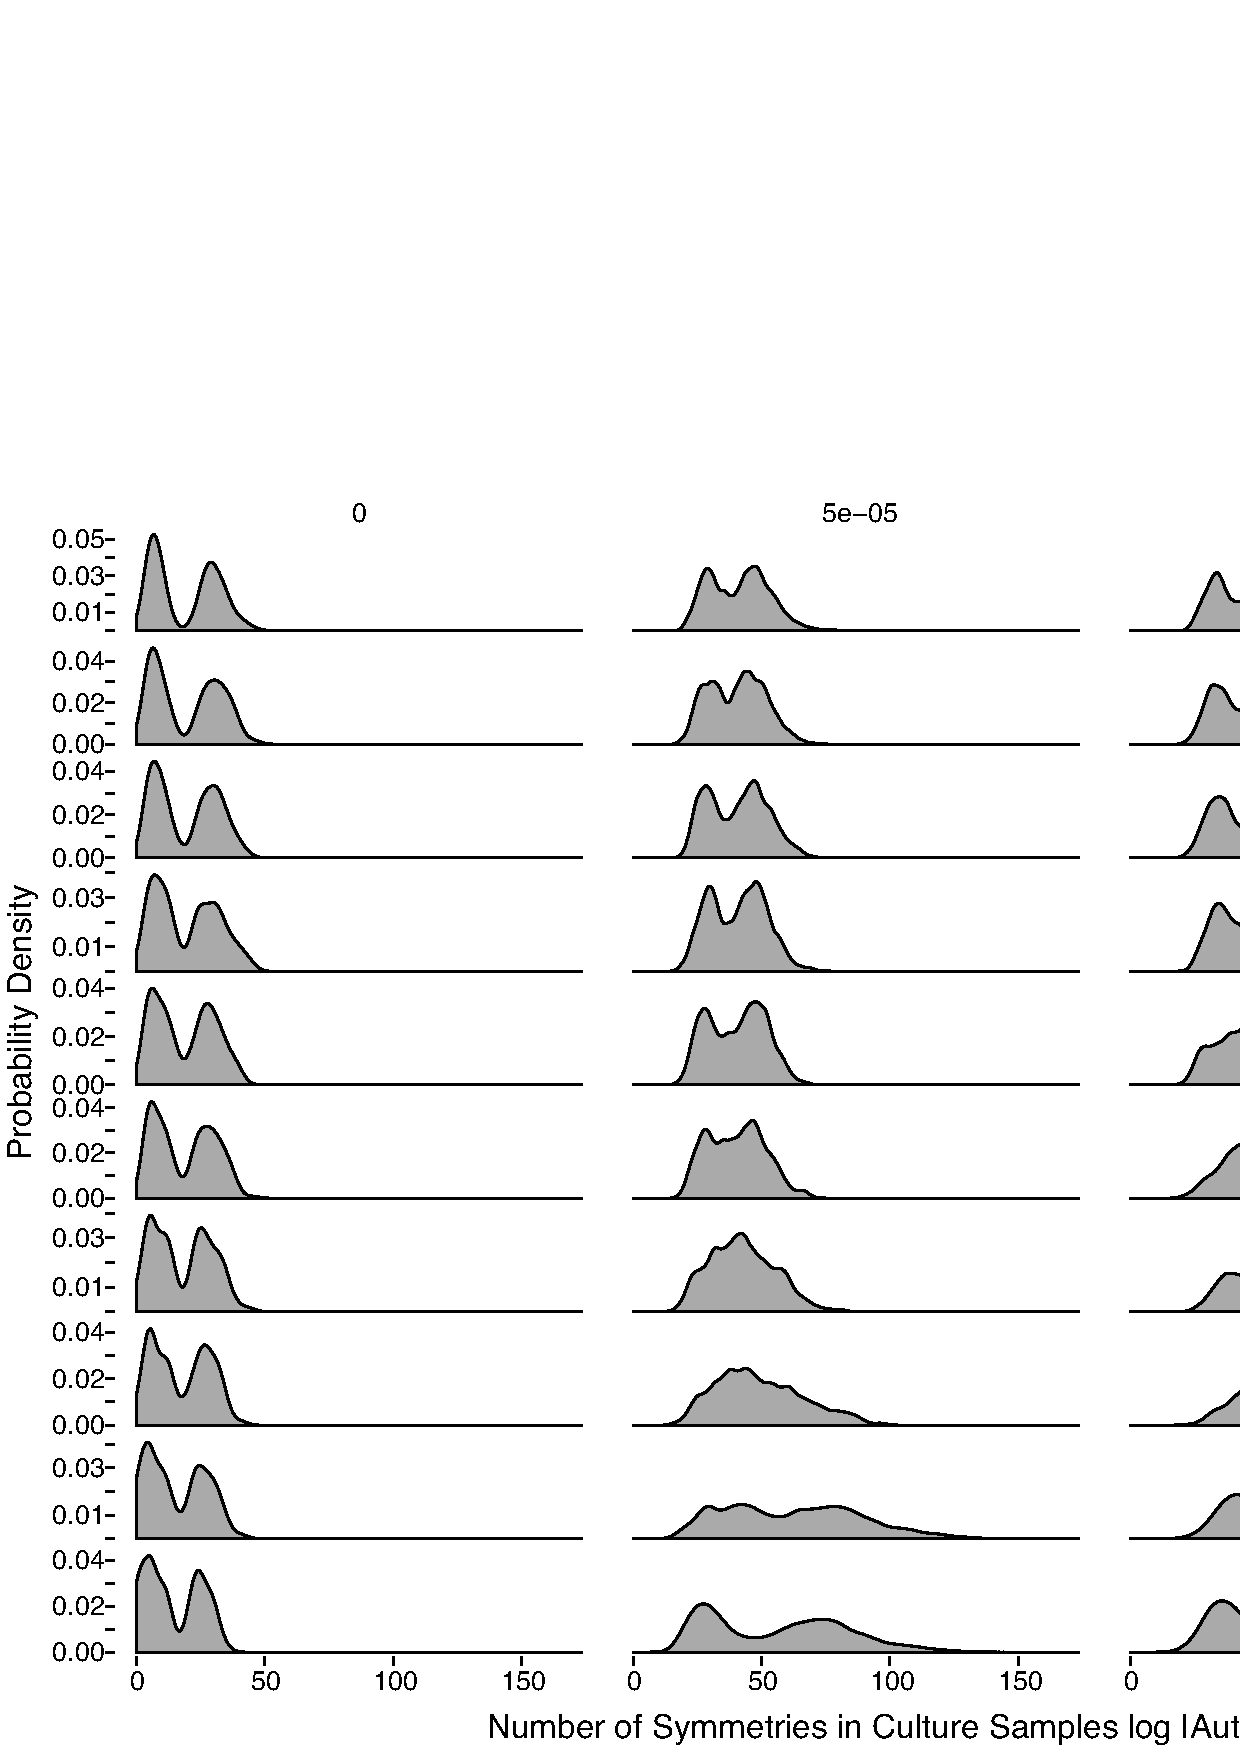
\includegraphics[scale=0.4]{autgroupsize-by-learning-by-innovation.pdf} 
\caption{Number of symmetries in trait tree samples, measured as the log of the order of the automorphism group of the trait graphs, broken down by prerequisite learning rate and global innovation rate.} 
\label{img:autgsize} 
\end{figure}

The logarithm of the automorphism group size does hint at interesting
structure (Figure \ref{img:autgsize}). In the presence of mutation, the
learning of prerequisites narrows the range of variability for the
automorphism group size, and at higher learning rates renders the
distribution multimodal. The modality arises because of the different
combinations of branching factor and depth factor we employed for design
spaces--i.e., some design spaces are ``wide'' and some are ``narrow,''
while also being ``shallow'' or ``deep.'' This gives rise to different
modes in the measured symmetries, but overall the reduction in
variability in symmetry is the most important qualitative effect seen in
our data.

We do not fully understand the ``shapes'' of cultural regions to which
the model appears to converge, but it appears that there is a tendency
for trait graphs to converge towards shapes which have moderate numbers
of symmetries. This graph is on a logarithmic scale, so a peak at 50
along the horizontal axis correponds to a trait graph with approximately
$5 \times 10^{21}$ symmetries. This is a fairly small number, compared
to the original design spaces, which have symmetries ranging from
approximately $10^{41}$ to $10^{6496}$. Thus, the geometry of cultural
traits in our hierarchical design spaces are fairly asymmetric and
represent small and very specific segments of the total design space.

Further analysis of trait graph ``shapes'' is needed to tell whether
there are repeating patterns or graph ``motifs'' which characterize a
social learning model in a graph-structured trait space. The results
here are suggestive of such a phenomenon, but inconclusive given just
the bulk algebraic properties of cultural regions, since the size of the
automorphism group (or the number of orbits) tells only \emph{how many}
symmetries there are, not what types of symmetries exist. The next step
in our analysis of shape is to pursue a geometric decomposition of the
graph following Ben MacArthur and
$\textrm{Rub\'en S\'anchez-Garc\'ia's}$
\citeyearpar{macarthur2008symmetry} work on the symmetries of complex
networks.

\section{Discussion}\label{discussion}

The ``semantic Axelrod'' model described here specifically addresses
social learning of knowledge with ``prerequisite'' structure, and a
learning environment which is tunable from low to high fidelity. We
introduced this model as a multifactor explanation for the transition in
the structure of social learning that may have occurred in early
\emph{Homo sapiens} and which has often been called the ``Upper
Paleolithic Transition'' or more neutrally, ``behavioral modernity.''

The model displays a characteristic increase in the cultural repertoires
of individuals, as they learn in environments of higher fidelity.
Individuals will tend to learn along ``pathways'' governed by the
knowledge of their models, elders, and peers, instead of the ``random
cultural samples'' they receive in a low-fidelity random copying
process. At the individual level, an increase in higher fidelity
learning within structured information environments both creates
path-dependency in what is learned, and increases the chances for
specialization among individuals. At the group and regional scale, we
expect that a metapopulation version of this model will display
regional-scale differences in cultural repertoires which become the
seeds for the persistent regional differences which characterize the
later Pleistocene and Holocene archaeological records.

The model described here only makes a start on modeling the additive and
recombinative complexity of real technologies, but it does display
accumulated depth of ``knowledge'' or ``skills,'' as represented by the
radius or depth of trait trees. In combination with realistic models of
technology--such as the production sequences studied by experts on stone
tools--we believe that empirically sufficient models of the evolution of
specific technologies are possible and within reach.

Several areas suggest themselves for future research in ``semantic''
Axelrod models. Some we are pursuing, others remain open questions and
we invite collaboration towards their solution.

\begin{itemize}
\itemsep1pt\parskip0pt\parsep0pt
\item
  Regional scale cultural differentiation given a metapopulation
  embedding of the basic model.
\item
  Additional trait relations (e.g., class subsumption, functional
  equivalencies).
\item
  Realistic technology models for key artifact classes (e.g., bifaces,
  scrapers, pottery).
\item
  Incorporation of trait fitness in order to study directional change.
\end{itemize}

We believe that models of the class studied here are a promising
platform for studying the effects of social learning of realistic
technologies that go beyond abstract, structureless ``tokens.'' Studying
the evolution of biological populations in detail eventually required a
detailed model of genomics beyond the ``bean-bag'' locus/allele models
of early theoretical population genetics \citep{mayr1959mayr}.\footnote{Although
  the controversy over ``bean-bag'' genetics is more complex than
  discussed here. See Ewens \citeyearpar{ewens2008commentary} for a
  contemporary commentary.} Going beyond the early promise of abstract
cultural transmission models and explaining real technological change
will require a similar transition beyond ``bean-bag'' social learning
models. We offer a small step in that direction.

\section{Acknowledgements}\label{acknowledgements}

The authors wish to thank Briggs Buchanan and Mark Collard for the
invitation to participate in the symposium ``Current Research in
Evolutionary Archaeology,'' at the 79th Annual Meeting of the Society
for American Archaeology in Austin, TX. A summary of this research was
presented in that session. Madsen wishes to thank
$\textrm{Fr\'ed\'eric}$ Chapoton of the Institut Camille Jordan for
answering a question about the maximal automorphism group of trees, and
Ben MacArthur and $\textrm{Rub\'en J. S\'anchez-Garc\'ia}$ for sharing
their geometric decomposition code.

\section{Appendices}\label{appendices}

\subsection{Algorithm Description}\label{algorithm-description}

Algorithm \ref{alg:tree-prereq-axelrod} describes the ``semantic'' Axelrod model variant studied in this chapter.  Within the algorithm, there are several functions which find traits with particular properties.  Some, like \textbf{GetTraitUniquetoFocal()}, are fairly simple set operations but were abbreviated to clarify the notation. 

\begin{algorithm}[H]
  \caption{}
  \label{alg:tree-prereq-axelrod}
  \begin{boxedminipage}{\textwidth}
  \begin{algorithmic}[1]
    %\REQUIRE lossrate is the population rate at which traits are randomly lost to drift
    \REQUIRE innovrate is the population rate at which individuals randomly learn a trait
    \REQUIRE learningrate is the probability of learning a missing prerequisite during a learning interaction

    \STATE { $focal \leftarrow$ GetRandomAgent()}
    \STATE { $neighbor \leftarrow$ GetRandomNeighbor(focal)}

    \IF { $focal = neighbor \lor focal \cap neighbor = \varnothing\;\lor  
    neighbor \subsetneq focal $}
    \label{alg:ext-first-if}
      \STATE { exit }
      \COMMENT{ No interaction is possible, move on to next agent }
    \ENDIF

    \STATE { $prob \leftarrow (focal \cup neighbor  - focal \cap neighbor) / focal \cup neighbor$ }

    \IF {RandomUniform() $< prob$}
      \STATE { $differing \leftarrow neighbor \setminus focal$ }
      \STATE { $newtrait \leftarrow$ GetRandomChoice(differing)}

      \IF {hasPrerequisiteForTrait($focal$, $newtrait$) = True}
        \STATE {$replace \leftarrow$ GetTraitUniquetoFocal(focal,neighbor)}
        \STATE { $focal \leftarrow focal \setminus replace$}
        \STATE { $focal \leftarrow focal \cup newtrait$}
      \ELSE
        \IF {RandomUniform() $< learningrate$}
          \STATE {$prereq \leftarrow$ GetDeepestMissingPrerequisite(newtrait, focal)}
          \STATE { $focal \leftarrow focal \cup prereq$ }
        \ENDIF
      \ENDIF

    \ENDIF
    %\IF {RandomUniform() $< lossrate$}
    % \STATE { $focal2 \leftarrow$ GetRandomAgent()}
    % \STATE { $loss \leftarrow$ GetRandomTrait(focal2)}
    % \STATE { $focal2 \leftarrow focal2 \setminus loss$}
    %\ENDIF

    \IF {RandomUniform() $< innovrate$}
      \STATE { $focal3 \leftarrow$ GetRandomAgent()}
      \STATE { $innovation \leftarrow$ GetRandomTraitNotInFocal(focal3)}
      \STATE { $focal3 \leftarrow focal3 \cup innovation$}
    \ENDIF

  \end{algorithmic}
  \end{boxedminipage}
\end{algorithm} 

\textbf{GetDeepestMissingPrerequisite()} is a procedure which takes the trait set of an individual, and a trait for which the individual is known to be missing necessary prerequisites, and returns the ``most basic'' missing prerequisite for that trait (i.e., closest to the root). This is done by finding the path which connects the root and desired trait, and walking its vertices from the root downward, checking to see if each vertex is part of the individual's trait set.  The first trait not found in the individual's repertoire is returned.  

\subsection{Availability of Software and Analysis
Code}\label{availability-of-software-and-analysis-code}

The software used in this chapter is available under an open-source
license at Mark Madsen's GitHub repository
\url{https://github.com/mmadsen/axelrod-ct}. Required libraries and
software are listed in the source archive itself, and include Python 2.7
and the open-source MongoDB database engine to store simulation output.

The codebase consists of a set of library modules which implement the
shared and unique aspects of each model, unit tests to verify the basic
functionality of the code, and scripts which execute each model. The
\textbf{axelrod-ct} repository contains three models:

\begin{itemize}
\item
  An implementation of the original Axelrod model using the
  \textbf{axelrod-ct} libraries.
\item
  A basic model with an ``extensible'' trait space but no relations
  between traits.
\item
  A ``semantic'' Axelrod model with tree-structured trait space
  representing prerequisite relationships between traits.
\end{itemize}

Stepwise extension from the original Axelrod to the semantic models on
the same code library allowed a degree of verification, which is
difficult in a situation where there is no existing mathematical theory
against which to compare the code implementation
\citep{national2012Assessing}.

The analysis and final dataset reported here are available, along with
the source of this paper and associated presentations, in an associated
GitHub repository: \url{https://github.com/mmadsen/madsenlipo2014}.
Statistical analyses of the final dataset were performed in R, employing
Knitr to render the results directly in publication format, and thus
reproducible by others \citep{xie2013dynamic}.


%% References with bibTeX database:

\bibliographystyle{model2-names}
\bibliography{madsenlipo2014-semanticaxelrod}

\end{document}
